\label{chapt:prelim}

In this section, the methods used for the numerical approach are discussed in detail. Parameters used in this section to follow Table~\ref{table:prelim_params}.

%----------------------------------------------------------------------------------------------------------------------
\section{Deflections \& Differential Relations}

The first equation that is presented is the main relation between the internal bending moment on a beam and its curvature by Equation~\ref{eq:Mcurve} as per \cite{nisbett2014shigley}. 

\begin{equation}
	\label{eq:Mcurve}
	\frac{1}{\rho}=\frac{M}{EI}
\end{equation}

Where $1/\rho$ is the radius of curvature defined as Equation~\ref{eq:curve} \cite{nisbett2014shigley}.

\begin{equation}
	\label{eq:curve}
	\frac{1}{\rho}=\frac{d^2y/dx^2}{\left( 1 +(dy/dx)^2 \right)^\frac{3}{2}} \approx \frac{d^2y}{dx^2}
\end{equation}

With \ref{eq:curve}, relations based on deflection $y(x)$ for slope \ref{eq:slope}, moment \ref{eq:mmt}, shearing force \ref{eq:shr} and load intensity \ref{eq:loadintens} as per \cite{nisbett2014shigley}.

\begin{equation}
	\label{eq:slope}
	\theta(x) = \frac{dy}{dx}
\end{equation}

\begin{equation}
	\label{eq:mmt}
	M(x) = EI\ \frac{d\theta(x)}{dx} = EI\ \frac{d^2y}{dx^2}
\end{equation}

\begin{equation}
	\label{eq:shr}
	V(x) = \frac{dM(x)}{dx} = EI\ \frac{d^3y}{dx^3}
\end{equation}

\begin{equation}
	\label{eq:loadintens}
	q(x) = \frac{dV(x)}{dx} = EI\ \frac{d^4y}{dx^4}
\end{equation}

\subsection{Boundary Conditions}

From these above equations, we may present boundary conditions (BC) as follows assuming that the boundary in question is located at $x_0$.\\

\textbf{Free Ends:}\\
\begin{equation}
	\label{eq:2_freeBC}
	\begin{aligned}
		y(x_0) = y_0          \\
		\theta(x_0)= \theta_0 \\
		M(x_0) = 0            \\
		V(x_0) = 0            
	\end{aligned}
\end{equation}

\textbf{Simply Supported:}\\
\begin{equation}
	\label{eq:2_endBC}
	\begin{aligned}
		y(x_0)= 0            \\
		\theta(x_0)=\theta_0 \\
		M(x_0)= 0            \\
		V(x_0) =V_0          
	\end{aligned}
\end{equation}

\textbf{Fixed:}\\
\begin{equation}
	\label{eq:2_fixedBC}
	\begin{aligned}
		y(x_0)=0      \\
		\theta(x_0)=0 \\
		M(x_0)=M_0    \\
		V(x_0) =V_0   
	\end{aligned}
\end{equation}

In the following section, these preliminary relations will be used to further expand on more complex analysis approaches.

%----------------------------------------------------------------------------------------------------------------------
\section{Theory of Cylindrical Shells}


As per Timoshenko's book \cite{timoshenko1959theory}, this section will cover the method of approximating the cylinder as a long thin shell. With this assumption, the governing ordinary differential equation (ODE) will be derived. The following coordinate system is presented as per Figure~\ref{fig:CoordSyst} below.

\begin{figure}[H]
	\centering
	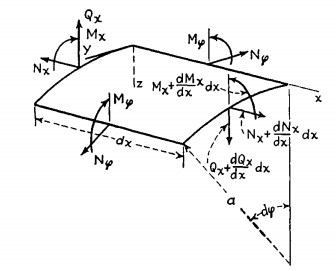
\includegraphics[width=0.6\textwidth]{CoordSyst}
	\caption[Coordinate system adopted for derivation of DEs.]{Coordinate system adopted for derivation of DEs.\protect\cite{timoshenko1959theory}}
	\label{fig:CoordSyst}
\end{figure}

Based on this, the following differential equations are presented as a pressure balance knowing that the differential area can be represented as Equation~\ref{eq:diffsurf}
 
\begin{equation}
	\label{eq:diffsurf}
	dA = dS\ dx = a\ d\varphi \ dx   
\end{equation}

The equations of equilibrium may be written as a force projection about the x and z axis and momment balance about y as Equations ~\ref{eq:eqbrm_x}, ~\ref{eq:eqbrm_z}, ~\ref{eq:eqbrm_y} respectively.

\begin{equation}
	\label{eq:eqbrm_x}
	\frac{dN_x}{dx}\ a\ d\varphi \ dx = 0
\end{equation}

\begin{equation}
	\label{eq:eqbrm_z}
	\frac{dQ_x}{dx}\ a\ d\varphi \ dx+ N_\varphi \ a\ d\varphi \ dx +Z\ a\ d\varphi \ dx= 0
\end{equation}

\begin{equation}
	\label{eq:eqbrm_y}
	\frac{dM_x}{dx}\ a\ d\varphi \ dx- Q_x\ a\ d\varphi \ dx= 0
\end{equation}

First looking at \ref{eq:eqbrm_x}, simplifying this equation and taking the integral with respect to $x$ will leave \ref{eq:eqbrm_x2}. 

\begin{equation}
	\label{eq:eqbrm_x2}
	N_x = C = 0 
\end{equation}

This above equation simply states that the effects of bending due to the axial forces will be neglected.\\

Similarly with \ref{eq:eqbrm_z} and \ref{eq:eqbrm_y}, simplifications will lead to \ref{eq:eqbrm_z2} and \ref{eq:eqbrm_y2} respectively.
\begin{equation}
	\label{eq:eqbrm_z2}
	\frac{dQ_x}{dx}+\frac{1}{a}\ N_\varphi = -Z
\end{equation}

\begin{equation}
	\label{eq:eqbrm_y2}
	\frac{dM_x}{dx}- Q_x= 0
\end{equation} 

With these equations and using strain relations from Hooke's law, the fine DE for displacement will be determined. In Equation ~\ref{eq:strain_xphi}, the relations between displacement and strain are presented.

\begin{equation}
	\label{eq:strain_xphi}
	\begin{aligned}
		\epsilon_x = \frac{du}{dx}      \\
		\epsilon_\varphi = -\frac{w}{a} 
	\end{aligned}
\end{equation}

From Hooke's law $N_x$ may be also written as Equation~\ref{eq:Hookes_Nx}. Substituting ~\ref{eq:strain_xphi} will leave the final simplification.
\begin{equation}
	\label{eq:Hookes_Nx}
	N_x = \frac{Eh}{1-\nu^2}\ \left( \epsilon_x + \nu \epsilon_\varphi \right) =  \frac{Eh}{1-\nu^2}\ \left( \frac{du}{dx} -\nu \ \frac{w}{a} \right)
\end{equation} 

%%tilde is UNBREAKABLE SPACE
Solving Equation~\ref{eq:Hookes_Nx} using ~\ref{eq:eqbrm_x2} leaves \ref{eq:Nx_simpl}.
\begin{equation}
	\label{eq:Nx_simpl}
	\frac{du}{dx} =  \nu \ \frac{w}{a}
\end{equation} 

Similarly, with $N_\varphi$, again applying \ref{eq:strain_xphi} leaves \ref{eq:Nphi_simpl}.
\begin{equation}
	\label{eq:Hookes_Nphi}
	N_\varphi = \frac{Eh}{1-\nu^2}\ \left( \epsilon_\varphi + \nu \epsilon_x \right) = \frac{Eh}{1-\nu^2}\  \left( -\frac{w}{a}+\nu \ \frac{du}{dx} \right)
\end{equation} 

\begin{equation}
	\label{eq:Nphi_simpl}
	N_\varphi = - \frac{Ehw}{a}
\end{equation}

As a result of no change in curvature in the $\varphi$ direction, we know that $\frac{dM_\varphi}{d\varphi}= 0$ hence no change in the circumferential moments. This relation is translated to axial momments $M_x$ with \ref{eq:Mphix}.

\begin{equation}
	\label{eq:Mphix}
	\begin{aligned}
		M_\varphi = \nu M_x        \\
		M_x = -D \frac{d^2w}{dx^2} 
	\end{aligned}
\end{equation}

Where $D$ is the flexural rigidity of the shell \ref{eq:flexrig}. This term replaces the $EI$ term from Equations~\ref{eq:Mcurve} - \ref{eq:loadintens}.

\begin{equation}
	\label{eq:flexrig}
	D \triangleq \frac{Eh^3}{12(1-\nu^3)}
\end{equation}

Simplifying \ref{eq:eqbrm_z2} to get $Q_x = \frac{dM_x}{dx}$, the following is put in \ref{eq:eqbrm_y2} to get \ref{eq:de1}

\begin{equation}
	\label{eq:de1}
	\begin{aligned}
		\frac{d^2M_x}{dx^2}+\frac{1}{a} \ N_\varphi = -Z \\
		D\ \frac{d^4w}{dx^4}+\frac{Eh}{a^2} \ w = Z      \\
		\frac{d^4w}{dx^4}+\beta^4 \ w = \frac{Z}{D}      
	\end{aligned}
\end{equation} 

Where $\beta^4$ is some parameter defined as \ref{eq:betaquad}.

\begin{equation}
	\label{eq:betaquad}
	\beta^4 \triangleq \frac{Eh}{4a^2D}= \frac{3(1-\nu^2)}{a^2h^2}
\end{equation}

The solution to this common fourth order, linear, non-homogeneous, ODE in \ref{eq:de1} has a general solution of Equation~\ref{eq:solnDE} \cite{timoshenko1959theory}.

\begin{equation}
	\label{eq:solnDE}
	w(x)=e^{\beta x} \left(C_1 \cos \beta x +C_2 \sin \beta x \right)+e^{-\beta x} \left(C_3 \cos \beta x +C_4 \sin \beta x \right) +f(x)
\end{equation}

Where $ C_1, C_2, C_3, C_4$ are integration constants to be solved based on BC and $f(x)$ is the particular solution to the ODE (recall $y_{general}=y_{homogeneous}+y_{particular}$).\\

In the following section, the exact solution to this differential equation given the loading scenarios in question.

%----------------------------------------------------------------------------------------------------------------------

\section{Application Solution}

With the previously developed equations and \cite{roarks}, the equations were solved using \cite{EXCEL}.\\

Calculated value of $t=1.686 in  = 42.8\ mm$

\section{Buckling}
\label{section:3_buckle}

Assumed linear buckling using Equations from Table 35 of \cite{roarks}, the following equations are presented. A thin tube under uniform external pressure will buckle as follows.

For Equation~\ref{eq:3_buckle1}.
\begin{equation}
	\label{eq:3_buckle1}
	q' =\frac{1}{4} \frac{E}{1-\nu^2} \frac{t^3}{R^3}
\end{equation}

The above equation is to be used for very long tubes with free ends \cite{roarks}. In other words, the length of the barrel $L$ must be greater the critical length calculated with \ref{eq:3_lcrit}.
\begin{equation}
	\label{eq:3_lcrit}
	L' = 4.90 R \sqrt{\frac{R}{t}}
\end{equation}

For the studied range of $t \in [0.05, 1.1) \Rightarrow L < L' \therefore$ Equation~\ref{eq:3_buckle2} must be used to calculate the critical buckling pressure.

\begin{equation}
	\label{eq:3_buckle2}
	q' =0.807\  \frac{Et^2}{LR}\  \sqrt[4]{\left( \frac{1}{1-\nu^2} \right)^3 \left( \frac{t}{R}\right)^2}
\end{equation}

With \ref{eq:3_buckle2} and the aforementioned thickness range, critical pressure values were computed with the \cite{PYTHON} script in Appendix~\ref{appendix:a4}. These results are displayed in the following plot (see Figure~\ref{fig:3_buckling}).

\begin{figure}[H]
	\centering
	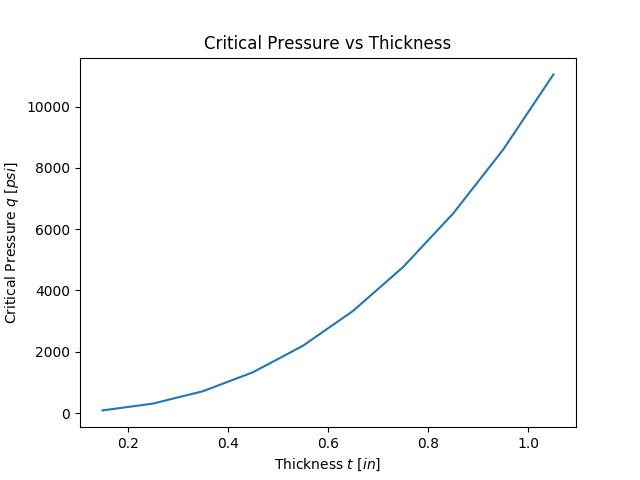
\includegraphics[scale=0.75]{3_buckling}
	\caption{Variation of critical buckling pressure $q'$ with thickness.}
	\label{fig:3_buckling}
\end{figure}

It is clear from above figure that a very low thickness is required to achieve a critical buckling pressure $q'$ of that in Equation~\ref{eq:2_preq} of $1376\ psi\ (9.484\ MPa)$. By rearranging, \ref{eq:3_buckle2} for $t$ and setting $q'=1376\ psi$, a critical thickness of $t=0.418\ in= 10.6\ mm$ is required to avoid buckling.\\

Based on the findings in this section, it is clear that buckling will not be the failure mode for this loading scenario.



